\section{Subject Behaviors}
\label{sec:subjectBehavior}

As stated: each Fully Specified Subject in a PASS model's Subject Interaction Diagram (SID) has at least one individual Subject Behavior Diagram (SBD) associated with it; it's base behavior\footnote{Macro and Guard Behaviors are described later.}. An SBD describes a subject's principle order of activities in a process context; it describes the subject's behavior. Therefore they describe and execution pattern or what to be done.  (in contrast to the SID that describes an interaction structure of active entities)

Note: SBD/states describe activities in principle and models necessarily needs to be aware of the execution he is implying. But the model and its execution are two related but different concepts. Be aware of what is talked about!

% The execution of the subject means sending and receiving messages and executing internal activities in the defined order. In the following sections, it is described what sending and receiving messages and executing internal functions means.

\subsection{States, Transitions, and Transition Conditions}
\label{sec:statesAndTransitions}

In principle, an SBD consist of \PASSModelElement{States} and \PASSModelElement{Transitions} used to describe what actions a subject performs in what order. To "be in a state" expresses that the subject is continuously performing the activity described on that state. The activity of state should be denoted at least by its label, but can also be detailed out with a \PASSModelElement{Function Specification}. One or more outgoing transition arrow denotes the next possible state to be executed as well as the condition (\PASSModelElement{Transition Condition}) that must be fulfilled in order to  follow the denoted path.  

\subsubsection{Do, Send, and Receive}

There are three principle state types in PASS: states that denote the execution of an internal action or function (\PASSModelElement{Do States}), and communication states to describe interaction with other subjects: This can either be the activity of sending a message to another subject (\PASSModelElement{Send States}) or the "activity" of waiting for and subsequently taking out a message from the inbox (\PASSModelElement{Receive State}).

Each state type corresponds with an according transition type: Send States with \PASSModelElement{Send Transitions}, Receive States with \PASSModelElement{Receive Transitions}, and Do States with \PASSModelElement{Do Transitions}. 

The Transition Condition to leave a Do-State via a Do Transition usually is that the activity is finished. In case there are multiple outgoing transitions, what the result or outcome of the activity was.

The Transition Condition to leave a Receive State is that a certain Message from a certain sending Subject is in the Inbox of a subject an can be taken out. The actual act of receiving is happening in the moment when following the transition. Before that, the activity of a receive state is, as stated, waiting. 

Finally, denoted on a Send Transition, the Transition Condition to leave a Send State is that a specified Message to a specified Receiving Subject has been sent. Before that, the activity of a Send State is concerned with the preparation of the Message. 

Figure \ref{fig:behavior-symbole} shows the different types of states with the corresponding symbols.

\begin{figure*}[htbp]
	\centering
	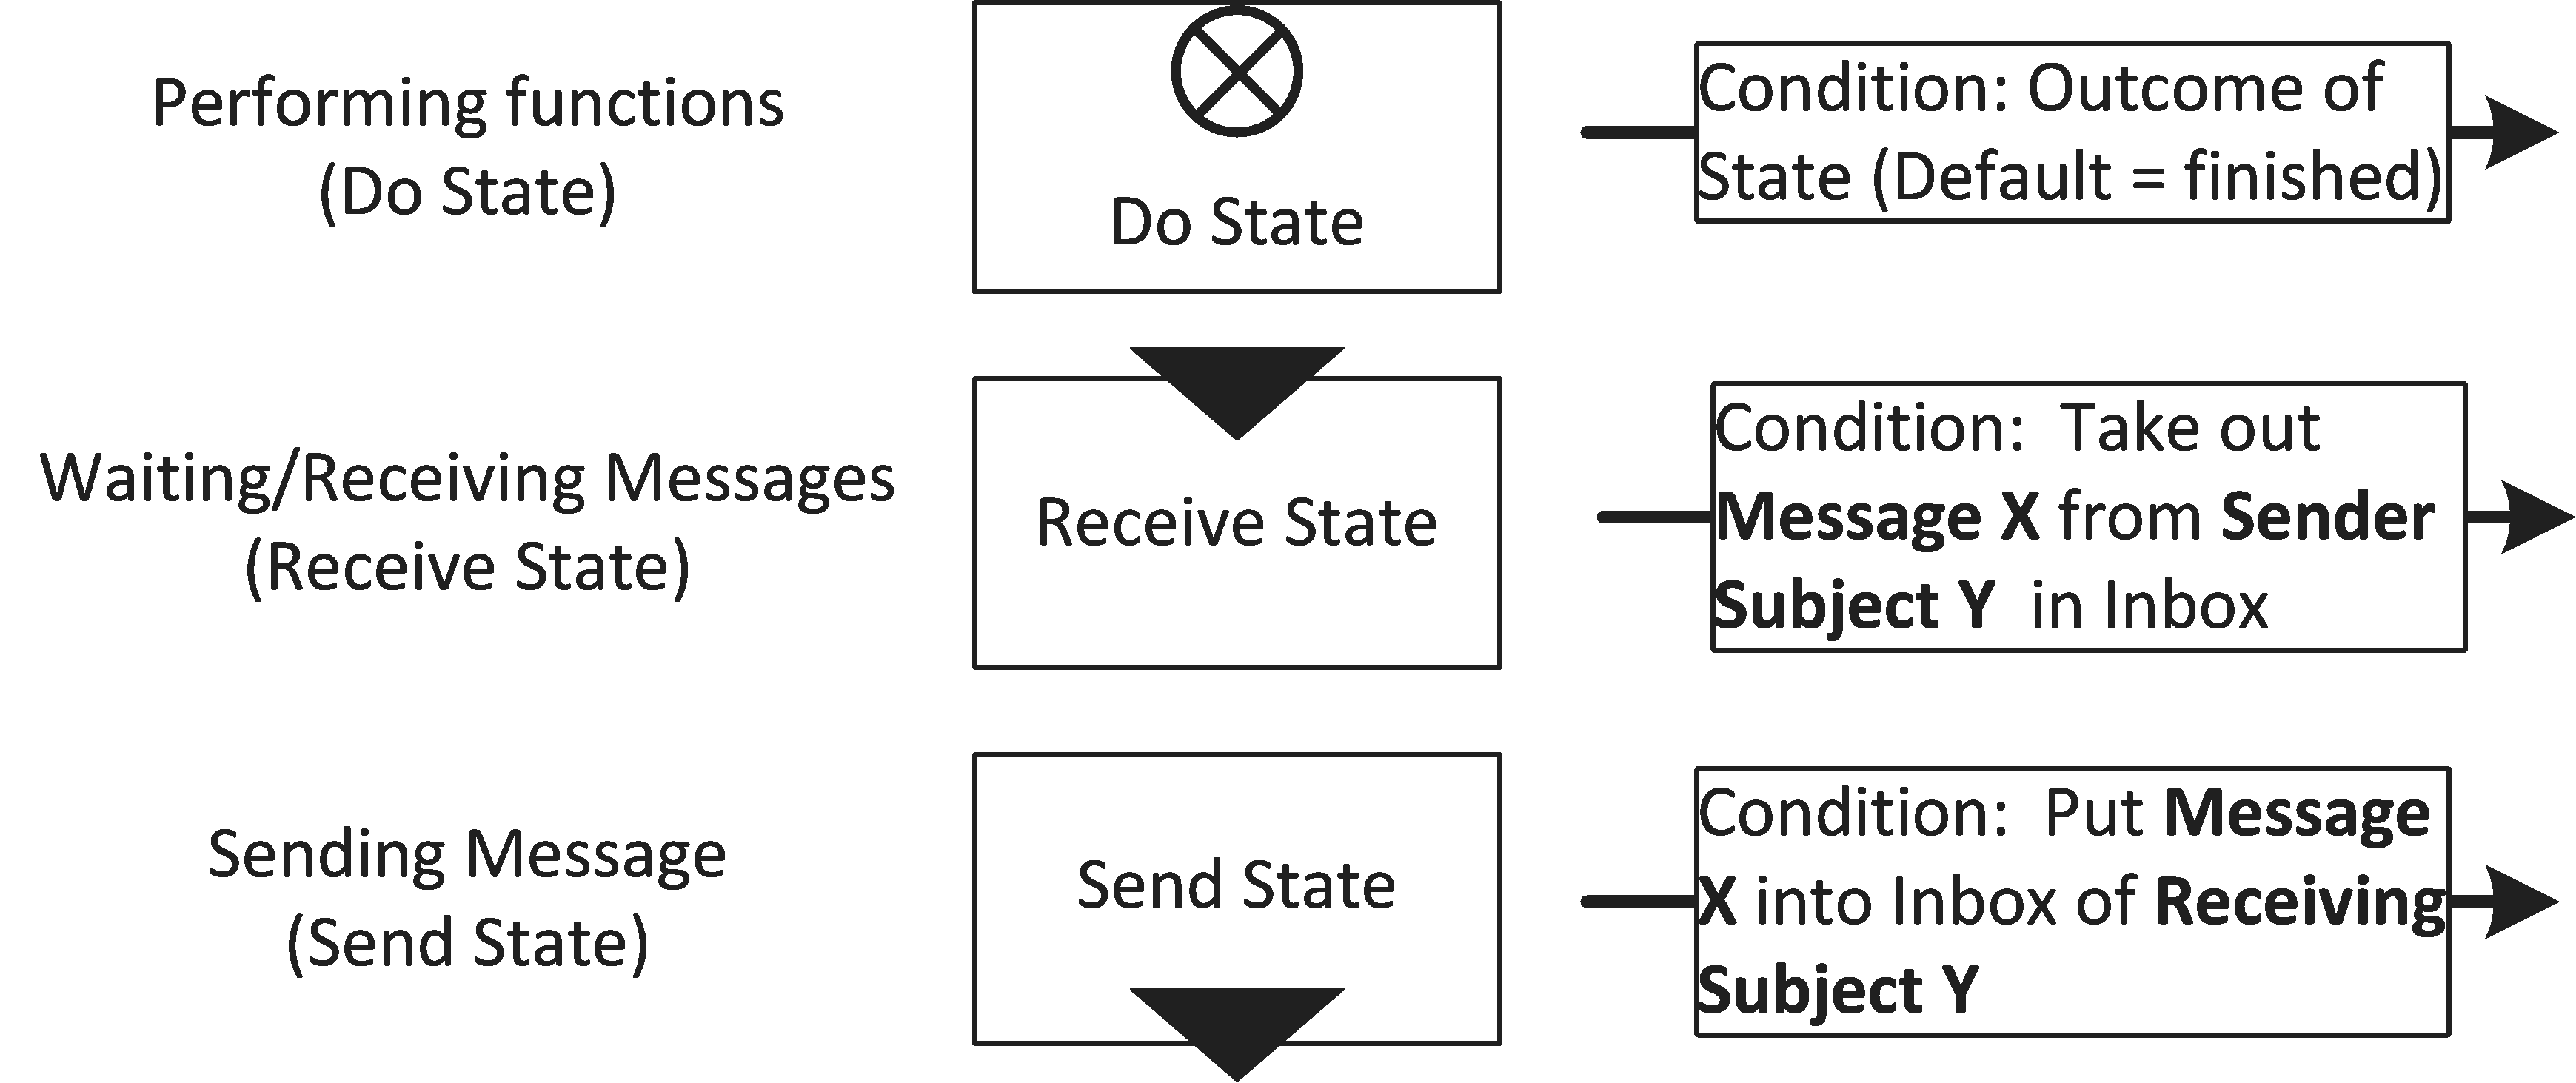
\includegraphics[width=0.9\linewidth]{Figures/Ontology/SubjectBehavior/Behavior-Symbole_NEW2.png}
	\caption[Symbols for the principle State types and corresponding Transition types in an SBD]{Symbols for the principle State types corresponding Transition types in an SBD}
	\label{fig:behavior-symbole}
\end{figure*}

\subsubsection{Send and Receive Types}
\label{sec:sendAndReceiveTypes}

The Transition Condition of Receive and Send Transitions can further be detailed out with a \PASSModelElement{Receive Type} or respective \PASSModelElement{Send Type}. These are important to define the interaction of the sending or receiving subject with multi-subjects.

By default the type of both is the standard type ( \PASSDefaultIndividual{Send Type Standard} and \PASSDefaultIndividual{Receive Type Standard}). This is intended for interaction with default \PASSModelElement{Single Subjects}, where in the context of a process model there will be a maximum of one interaction partner subject. In that case, it is expected that a message is send to or received from that interaction partner. If no instance of the partner Subject exist, such an instance will be created. This is different if the partner Subject is a \PASSModelElement{Multi-Subject}, implying that there can be multiple communication partners.\footnote{Reminder: the Multi Subject is a subject without Instantiation Restrictions, while it is the Single Subject is limited to be instantiated only once in a process context. See also Section \ref{sec:modelSubjectInstance} for the Concept of Subject Instances} 

In that case, for a Send Transition it can be specified that copies of message-to-be-send either to all known instances or to a \textbf{certain number} of instances  (\PASSDefaultIndividual{Send Type Multi Send To All} [known] or \PASSDefaultIndividual{SendTypeMultiSendToKnown}). Alternatively, it can be specified that the sending of this message is supposed to go to (or to create) a specified number of new subject instances (\PASSDefaultIndividual{SendTypeMultiSendToNew})

The other way around, when receiving from a Multi-Instance-Subject, it can be specified for the Transition Condition for a Receive Transition is not the reception of a single Message, but rather multiple copies of the same Message must be received. Either a \textbf{specified number} of messages from the known subject instances (\PASSDefaultIndividual{ReceiveTypeMultiReceiveFromKnwon}) or simply each known subject must have answered (\PASSDefaultIndividual{ReceiveTypeMultiReceiveFromAllKnown}).


\subsubsection{Start States}
\label{sec:startStates}

In each Behavior Diagram there is one and only one state that is denoted as the \PASSModelElement{Initial State Of [a] Behavior} or \textit{"Start State"}. And a subject is expected to be in that state upon initialization. 

If the Start State of an SBD is a Do State or a Send State the subject is expected to be active upon initialization of the overall process system out of its own accord. This can be denoted in the SID by marking the Subject as Start Subject (See section \ref{sec:startSubject}).

All other Subjects are expected to have a Receive State as the Start State of their SBD and therefore being initialized when another Subject send a message to them for the first time.

\subsubsection{End States}
\label{sec:endStates}

Any Do State and any Receive State of an SBD can be denoted to be an \PASSModelElement{End State} and all state-transition paths in an SBD should lead from the Start State to an End State. There can be multiple End States and a State is allowed to be starting and End State at the same time if the behavior is cyclic. 

If a Subject Instance is in an End State its execution can be \textit{terminated} permanently by a surrounding process execution system, however termination should only be done if all Subjects in a process context are in an End state during execution. Therefor it is possible to "reactivate" as subject. If the End State is a Receive State this is done via the sending of message received via a Receive Transition leaving that End State. If the End State is a Do State, denoting the the internal activity currently is "Do Nothing", the subject can be reactivated by that subject's carrier (See section \ref{sec:subjectCarrier}) on its own  via an outgoing Do Transition or User-Cancel. Alternatively, a Time Transition can be used to trigger a temporal condition to leave either Receive End States or Do End States.

\PASSModelElement{Send States} must not be declared to be End States! Being "in a state" means the activity, in that case sending, is not yet finished. However, sending is a explicit activity of informing someone else and should be finished upon the end of process. There simply is no point to model an sending activity without completing it. 

\subsubsection{Example for Complete Behavior Diagram}

Figure \ref{fig:vollst-beispiel} shows the Subject Behavior Diagrams of the Subjects 'employee', 'manager', and 'travel office' in the sample "Business Trip Application" process who's SID was introduced in  figure \ref{fig:beispiel-SubjectInteraction}:

\begin{landscape}
	\begin{figure}[htbp]
		\centering
		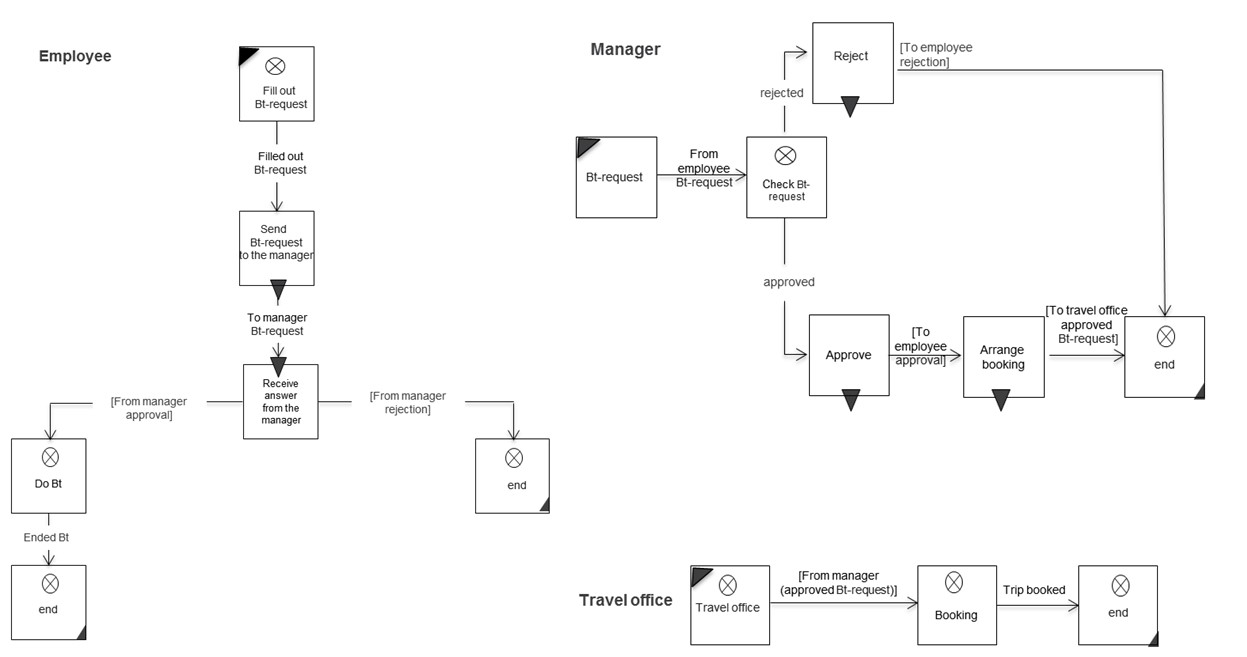
\includegraphics[width=0.9\linewidth]{Figures/Ontology/SubjectBehavior/Vollst-Beispiel}
		\caption[Subject Behavior Diagrams for the subjects 'employee', 'manager', and 'travel office' from figure \ref{fig:beispiel-SubjectInteraction}]{Subject Behavior Diagrams for the subjects 'employee', 'manager', and 'travel office' from figure \ref{fig:beispiel-SubjectInteraction}}
		\label{fig:vollst-beispiel}
	\end{figure}
\end{landscape}

In the depicted sample process, employees send completed requests using the message 'business trip request' to the manager's input pool. Upon reception, the manager checks the request and can either reject it and send the according message, or he can approve it. In the later case he must send the 'Approval' reply to the employee and forward the 'Approved Business Trip Request' to the travel office. It does not matter which message is attempted to be sent first. If the send mechanism is successful, the corresponding state transition is executed. 


\subsection{Branching \& Priorities}

\PASSModelElement{Send States} may have only one outgoing Send Transition! In contrast, \PASSModelElement{Do States} may have multiple outgoing \PASSModelElement{Do Transitions} and \PASSModelElement{Receive States} may have multiple outgoing \PASSModelElement{Receive Transitions}, creating branches or splits in the possible process paths. 

Since a subject is not a quantum particle it can be only in one \PASSModelElement{State} at once, therefore all branching in an SBD is always of exclusive alternative (X-OR) nature; there are no explicit AND- or OR-Splits and Joins in PASS.  However, there is a pseudo-AND spit in the form of the \PASSModelElement{Choice Segment} (See section \ref{sec:choiceSegement}).

For parallel executed activities (AND-Splits) the subject-oriented \textbf{Parallel} Activity Specification Schema (PASS) requires two or more different active entities (Subjects) to be modeled, that can work in parallel. Therefore a Send State/Transition combo leading to anything but a receive state waiting for direct answer to the sent message is basically an AND-Split while waiting for a corresponding message in a receive state is an AND-Join. 

For the case that the conditions of more than one outgoing transition of a state are fulfilled at the same time, each transition has a Priority Number to define a precedence order for choosing one of the valid paths. The PASS standard defines a lower Priority Number to be the higher priority (Priority Number "one" is higher than priority number "five"). If no such clear precedence order is defined and more than one transition condition is true, the path may be chosen a arbitrarily or at random.

\subsection{Further SBD Elements}

In addition to the core states and transitions, a Standard PASS SBD may contain a few other elements: User Cancel Transitions, Time Transitions, Sending Failed Transitions, and Choice Segments. 

\subsubsection{User Cancel}

A \PASSModelElement{User Cancel Transition} usually denotes the possibility to exit a receive state without the reception of a specific message. Basically, it allows for an arbitrary decision by a subject carrier/processor (See section \ref{sec:subjectCarrier}) to abort a waiting process.

In the example shown in Figure \ref{fig:receivestatebreak}, the receiving state can also be left to send an additional inquiry message. That message, necessarily, must have been defined in the according SID first.

\begin{figure*}[htbp]
	\centering
	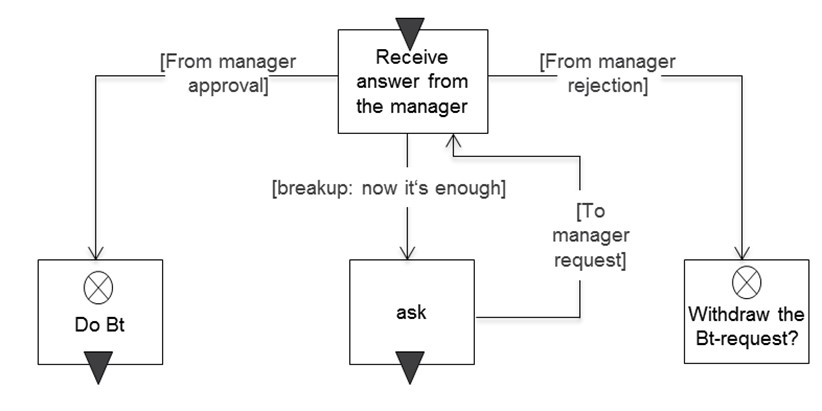
\includegraphics[width=0.7\linewidth]{Figures/Ontology/SubjectBehavior/ReceiveStateBreak}
	\caption[Message reception with User Cancel Transition]{Message reception with User Cancel Transition}
	\label{fig:receivestatebreak}
\end{figure*}

User Cancel Transitions could also originate from Do States, but here they are not very different from a normal Do-Transition and only emphasise the option to arbitrarily abort the execution of \PASSModelElement{Do Function Specification}, including the specification of what happens afterwards. 

It is also possible to attach a User Cancel to a Send State giving the subject carrier the option not to send the defined message but skip to another state. 

\subsubsection{Time Transitions}

Instead of having the decision to skip waiting or abort an activity left to the arbitrary decision of a subject carrier, Time Transitions can be used to model that a state transition should happen based on a time based constraint. 
There are to principle types of Time Transitions: Timer Transitions and Reminder Transition.

\PASSModelElement{Timer Transitions} basically denote time-outs for the state they originate from.  The condition for a Timer Transition is that a certain amount of time has passed since the state it originates from has been entered and thus starting the timer.

There are three variations for the Timer Transition based one the unit of time necessary to model them for. First is the \PASSModelElement{Day Time-Timer Transition} allowing to specify a time-out after a certain amount of Seconds, Minuets, or hours. This is the most basic Timer and shown in figure \ref{fig:receivestatetimer} where after waiting three days for the manager's answer, the employee sends another inquiring request.

\begin{figure*}[htbp]
	\centering
	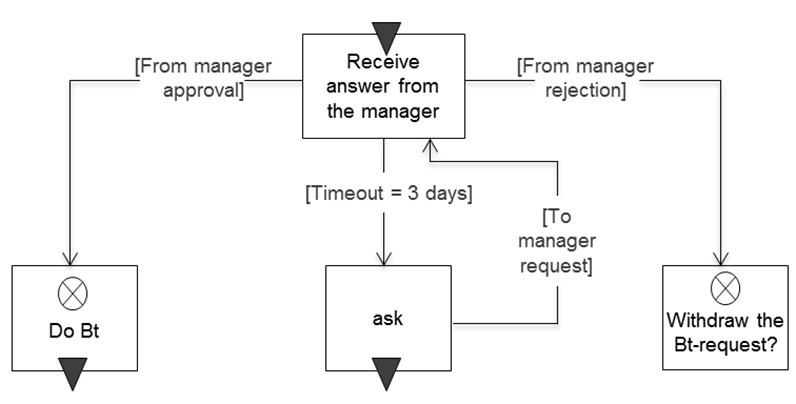
\includegraphics[width=0.7\linewidth]{Figures/Ontology/SubjectBehavior/ReceiveStateTimer}
	\caption[Time monitoring for message reception]{Time monitoring for message reception}
	\label{fig:receivestatetimer}
\end{figure*}

Due to difference and complication with measuring time calendarial (e.g. leap year concerns, leap seconds, different calendar systems), Time Transition based on years or months need to be different, following the XML standard for noting done time intervals ( \PASSModelElement{Year Month Timer Transition})

Finally as PASS is often used to model business processes, it is useful to be able to define a time-out after a certain amount of business days have passed, with the definition of business days depending the time the business process is executed and/or the legally binding geographical location of the executing instance (Business Day Timer Transition).

\PASSModelElement{Reminder Transitions} are transitions that can be traverses if a certain time based event is triggered, e.g. a certain calendar date has been reached, or frequency condition is met  since the last traversal of that transition (e.g. once per day).

As with the Timer Transition, the exact time definition can again either be based on calendarial consideration (\PASSModelElement{Calendar Based Reminder} Transition) or be based on hours, minuet, or seconds (\PASSModelElement{Time Based Reminder Transition}).


\subsubsection{Sending Failed Transition}

A \PASSModelElement{Sending Failed Transition} is a technical model element and can only originate from a send state. It is similar to a Time-Out Transition or User-cancel. It is used to denoted an alternative route from a send state if the process execution environment is not able to actually perform the implicated sending activity and thus fulfill the Transition Condition

\subsubsection{Choice Segments and Choice Segments Paths}
\label{sec:choiceSegement}

As stated before, the behavior of subjects is regarded as a distinct sequence of internal functions, as well as send and receive activities. Usually the order of the activities is either important and therefor modeled with consideration or the order does not matter and the modeler simply can arbitrarily choose a sequence. However, there are some cases where it is important to allow the order of execution of some states to be up to the choice of the subject carrier.

The freedom of choice with respect to behavior is described as a collection alternative paths in a so called \PASSModelElement{Choice Segment}. Each \PASSModelElement{Choice Segment Path} can be modeled to be optional or mandatory to start (\PASSModelElementDataAttribute{isOptionalToStartChoiceSegmentPath}), as well as separately optional or mandatory to end (\PASSModelElementDataAttribute{isOptionalToEndChoiceSegmentPath}. This leads to the following combinations.

\begin{itemize}
	\item Beginning is mandatory/end is mandatory: All states in a path need to be processed to the end.
	\item Beginning is mandatory/end is optional: The path alternative must be started (first state), but does not need to be finished. 
	\item Beginning is optional/end is mandatory: if the path is started, all states in the path must be completed.
	\item Beginning is optional/end is optional: path is completely optional
\end{itemize}

Note that state transitions in a Choice Segment Path must not point to states outside of the path. An alternate sequence starts in its start point and ends entirely within its endpoint.

The execution of a Choice Segment is considered complete when all mandatory to start paths have started and all mandatory to end paths have been entirely processed and have reached the end operator of that path.

Figure \ref{fig:alternative} shows an example for modeling Choice Segments. After receiving an order from the customer, three alternative behavioral sequences can be started, whereby the leftmost sequence, with the internal function 'update order' and sending the message 'deliver order' to the subject 'warehouse', must be started in any case. This is determined by the 'X' in the symbol for the start of the alternative sequences (the gray bar is the starting point for alternatives). This sequence must be processed through to the end of the alternative because it is also marked in the end symbol of this alternative with an 'X' (gray bar as the endpoint of the alternative).

\begin{figure}[htbp]
	\centering
	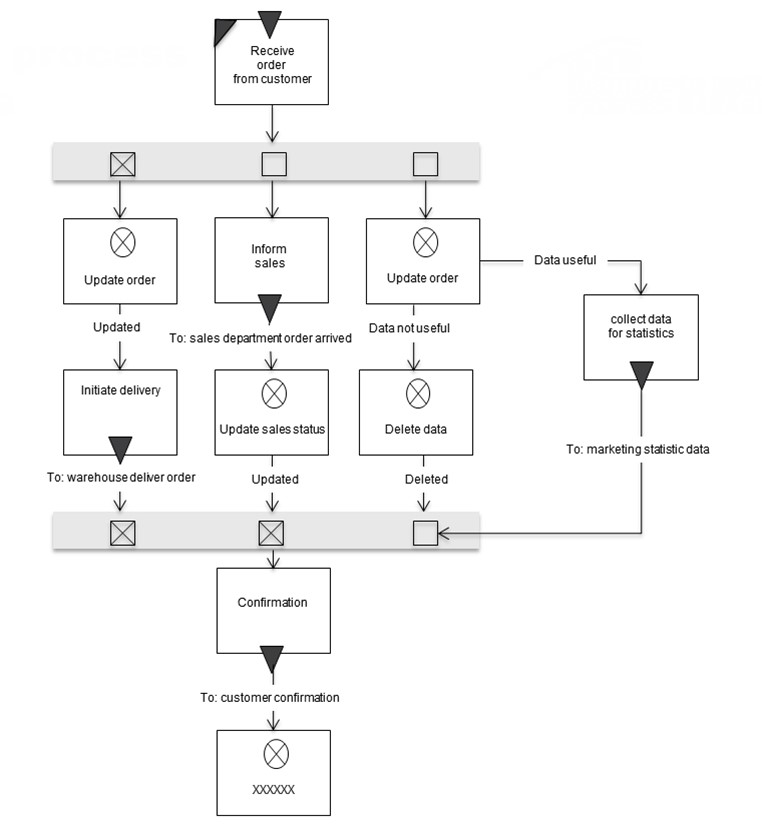
\includegraphics[width=0.7\linewidth]{Figures/Ontology/SubjectBehavior/ALternative}
	\caption[Example of a Choice Segment with three Choice Segment Paths]{Example of a Choice Segment with three Choice Segment Paths}
	\label{fig:alternative}
\end{figure}

The other two Choice Segment Paths can, but do not have to be, started. However, in case the middle path is started, i.e., the message 'order arrived' is sent to the sales department, it must be processed to the end. This is defined by an appropriate marking in the end symbol of the alternatives ('X' in the lower gray bar as the endpoint of the alternatives). The rightmost path is completely optional.

For the detailed execution semantic of the Choice Segment refer to section \ref{sec:choiceSegmentExecution}.

\subsubsection{The Action-Concept as an SBD element}

An \PASSModelElement{"Action"}, as an element of an SBD-model, simply is a grouping concept that groups a State with all its outgoing valid Transitions. This element rarely has visual representation in visual PASS modeling.

\section{Multiple Behaviors}
\label{sec:multipleBehaviors}

The default concept of PASS is, that for a Fully Specified Subject, there is one Subject Behavior Diagram --- the \PASSModelElement{Subject's Base Behavior}. However, for advanced modeling purposes standard PASS allows to add additional, special-purpose behaviors to a subject.
--- \PASSModelElement{Guard Behaviors} or \PASSModelElement{Macro Behaviors}. 

In principle, both, a Guard Behavior, or a (subject specific) Macro Behavior, are individual SBDs that are linked to a subject within the same overall PASS model. The communication capabilities in the additional SBDs are still determined by the same SID. 

A subject with multiple behaviors, still always \textit{is} in one State, however that state may be in one of the different behaviors. This implies that the currently \textit{"active"} behavior is changing over the course of the execution of a process model. As a consequence, it is necessary to determine a precedence order between them, to define which Behavior is responsible for a subject's actions if more than one Behavior could potentially be executed at the same time. For that purpose each Behavior \PASSModelElementDataAttribute{has [a] Priority Number} assigned to it, with the Base Behavior having the lowest priority in form of the highest Priority Number. The concept is, that different behaviors are laying "on top" of each other, forming a kind of "behavior stack" in the order of the priority numbers. 

\subsection{Switching Between Behaviors}
\label{sec:stateRef}

At least for an executable Base Behavior, as stated, it is expected that all the  states  are in a valid path between a Start State and a valid End State.

In Guard Behaviors there does not necessarily need to be an end in an End State, but there can be. Macro Behaviors \textbf{must not have an} \PASSModelElement{End State}!

Rather, they end in states that refer back to another Behavior to continue the execution there. The referred-to behavior, most likely, is the Base Behavior. 

There are two principle ways to refer back to another behavior First there is the specific \PASSModelElement{State Reference}; a kind of "state" that refers to a state in another behavior. A transitions leading to such a State Reference "state" is akin to that transition leading to the original state.

The second option is the \PASSModelElement{Generic Return-To-Origin-Reference}.

Both reference types must not be used in a Base Behavior, they are used under the assumption that the behavior they are used belongs to a model with multiple behaviors and in was entered from a Base Behavior. Either by Macro-Call from a state there, or because the reception of an Interrupt Message has triggered the Guard Behavior. 

%\footnote{The 1:1 relation between a subject and a behvior is very good concept. The concept of Abstract layered PASS (ALPS) \cite{elster:layer} trys to uphold it, even in situations with}

%\subsection{Extended Behavior}

%To reduce description efforts some additional specification constructs have been added to PASS. These constructs are informally explained in the following sections. 

\subsection{Guard Behaviors: Exception or Interrupt Handling} 

Normally, a subject can receive message only in according receive states. However, sometimes there are urgent messages that need to be handled out of order.

For example in the business trip booking process, if there is an additional message from another subject that can make the Employee cancel all the previously made plans, no matter at what point in the process he is.

From communication point of view, this is exemplaryily shown in Figure \ref{fig:sid-exception} where the concept is, that the newly introduced Service Cancellation Message can arrive arbitrarily at any point in time.

\begin{figure}[ph!]
	\centering
	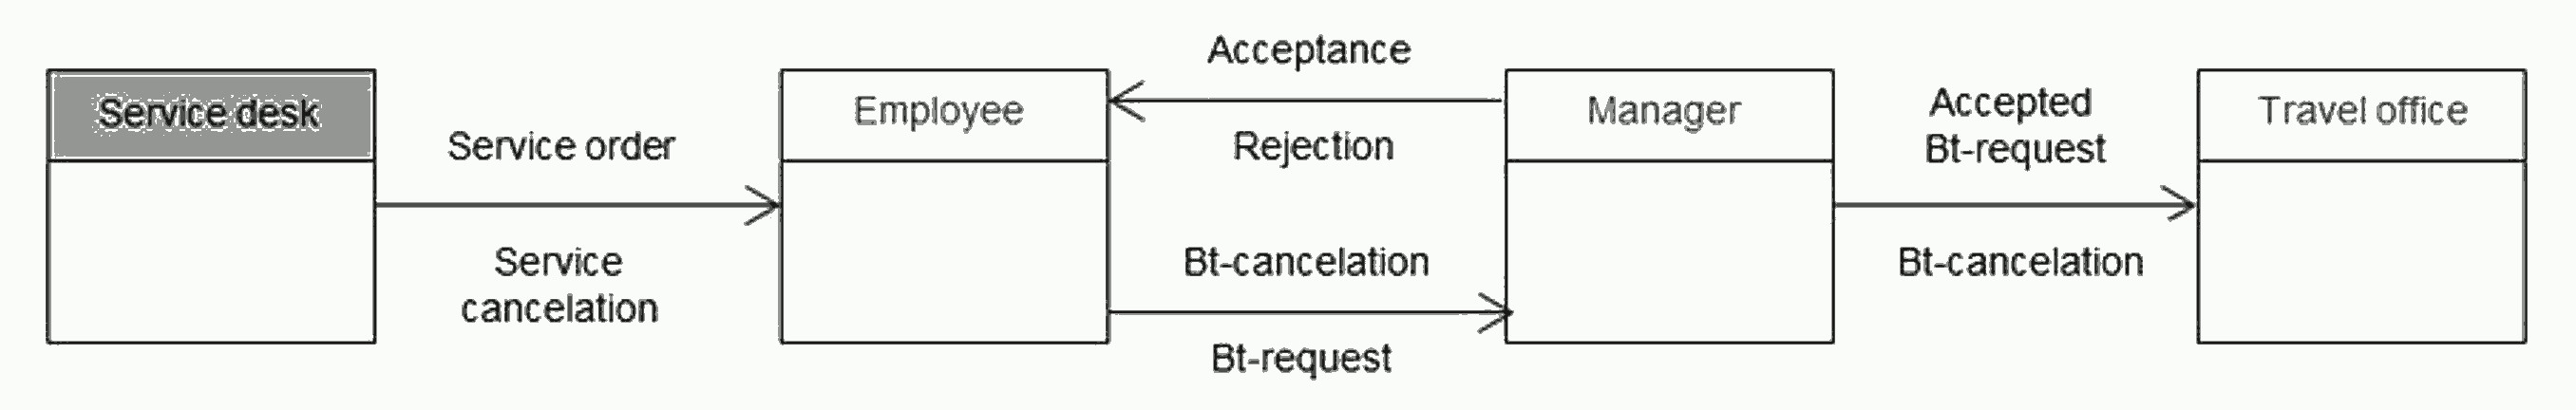
\includegraphics[width=0.9\linewidth]{Figures/Ontology/SubjectBehavior/SID-Exception}
	\caption[Extended SID of the business trip application with additional cancellation message from a Service Desk]{Extended SID of the business trip application with additional cancellation message from a Service Desk}
	\label{fig:sid-exception}
\end{figure}

With only one behavior and the classical means, handling of this message can only be done in the normal receive states as an alternatives, as shown in Figure \ref{fig:exceptionhandling}. Here, the Cancellation message may be handled the earliest after the original request was filled out or after it was send of to the manager, but not after the manager has send the acceptance notice, even if the trip could be canceled afterwards.


\begin{figure}[htbp]
	\centering
	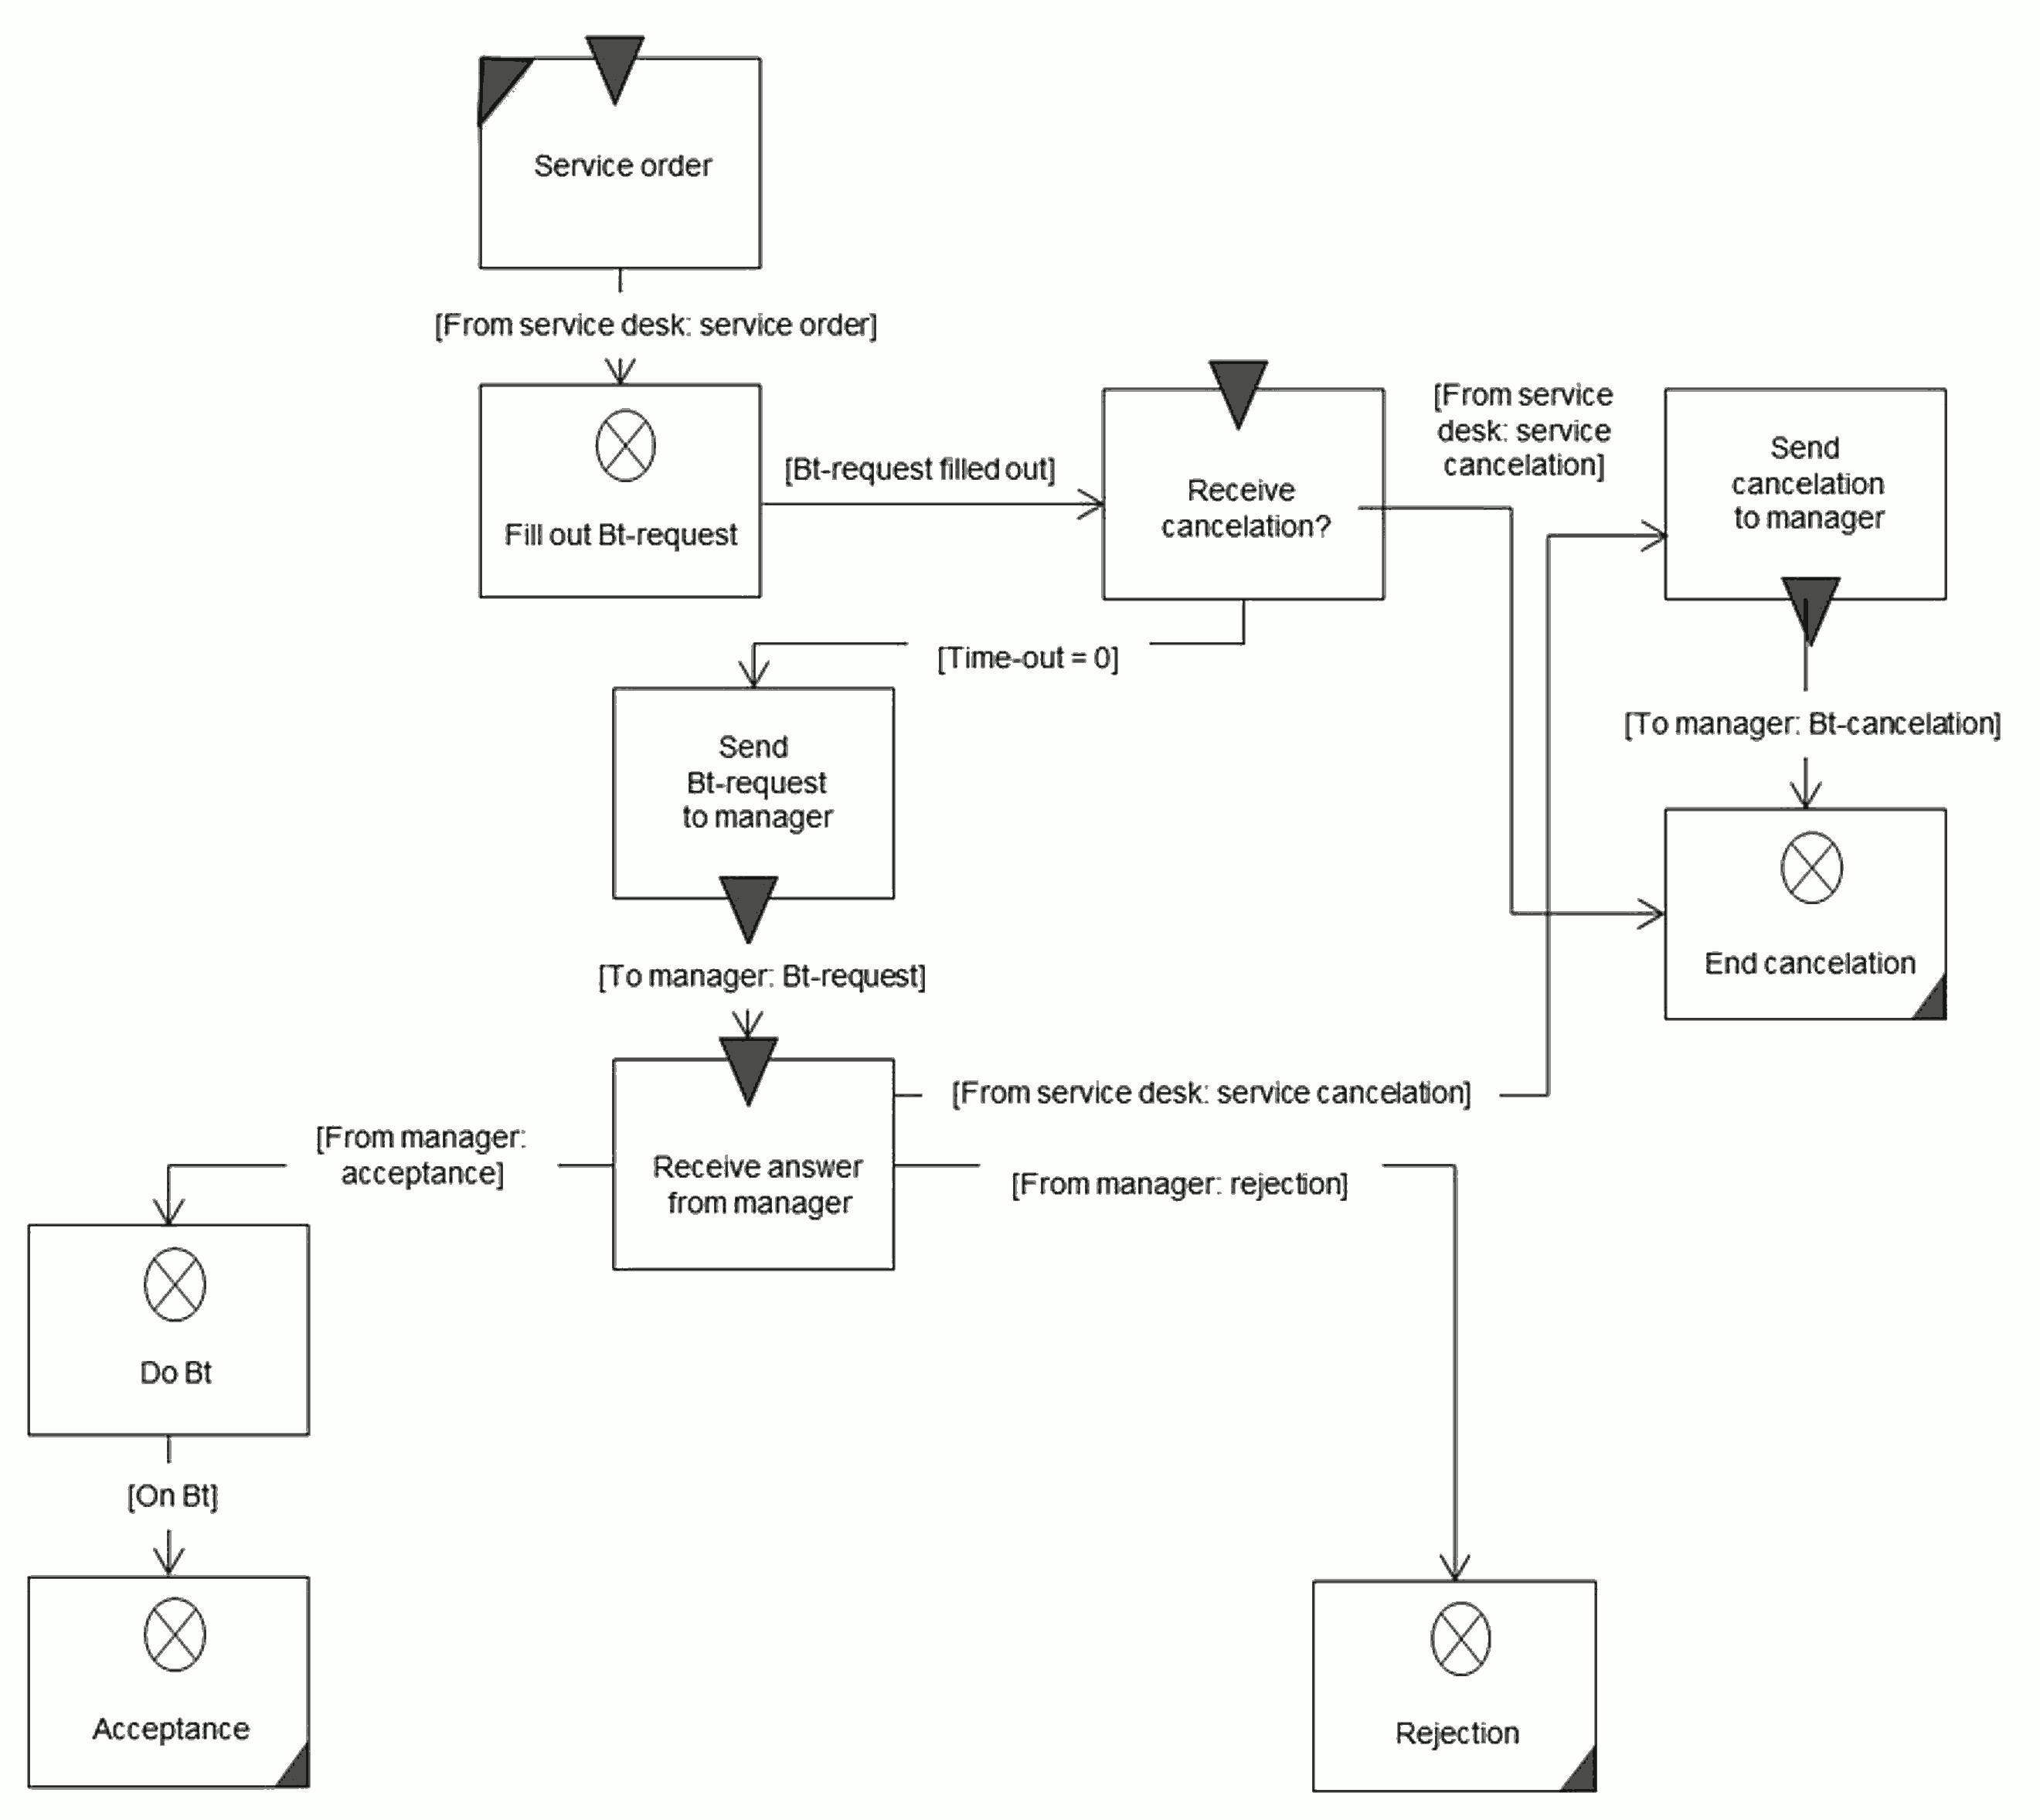
\includegraphics[width=0.7\linewidth]{Figures/Ontology/SubjectBehavior/ExceptionHandling}
	\caption[Handling the Cancellation Message using only standard SBD constructs]{Handling the Cancellation Message using only standard SBD constructs}
	\label{fig:exceptionhandling}
\end{figure}

Instead, the mechanism of the \PASSModelElement{Guard Behavior} can be used to model that some specific or all states of a Base Behavior are \textit{"guarded"} by another behavior. A Guard Behavior is a separate SBD that always has a Receive State as its initial state. All Messages that are received in such an initial state of Guard Behavior basically become interrupts or exceptions to the normal flow of the process. Upon the reception of such an Interrupt Message the subject \textit{"jumps"} to that initial state of the Guard Behavior and the process flow continues from there. The flow in a Guard Behavior may either lead to an End State, to a specified state that is referenced in the Guard Behavior, or the process flow can be set to continue where it left off, before switching to the execution of the Guard Behavior (See State Reference or Generic Return-To-Origin-Reference in section \ref{sec:stateRef}). For the whole concept to be specified properly,  the Guard Behavior must be set to either guard a specific State (\PASSModelElementObjectPropertie{guardsState}) or a complete Behavior (\PASSModelElementObjectPropertie{guardsBehavior}). Also, the Priority of the Guard Behavior must be higher than that of the guarded Behavior. 

Figure \ref{fig:extension1} shows such the multiple Behaviors for the subject Employee. 

\begin{figure}[htbp]
	\centering
	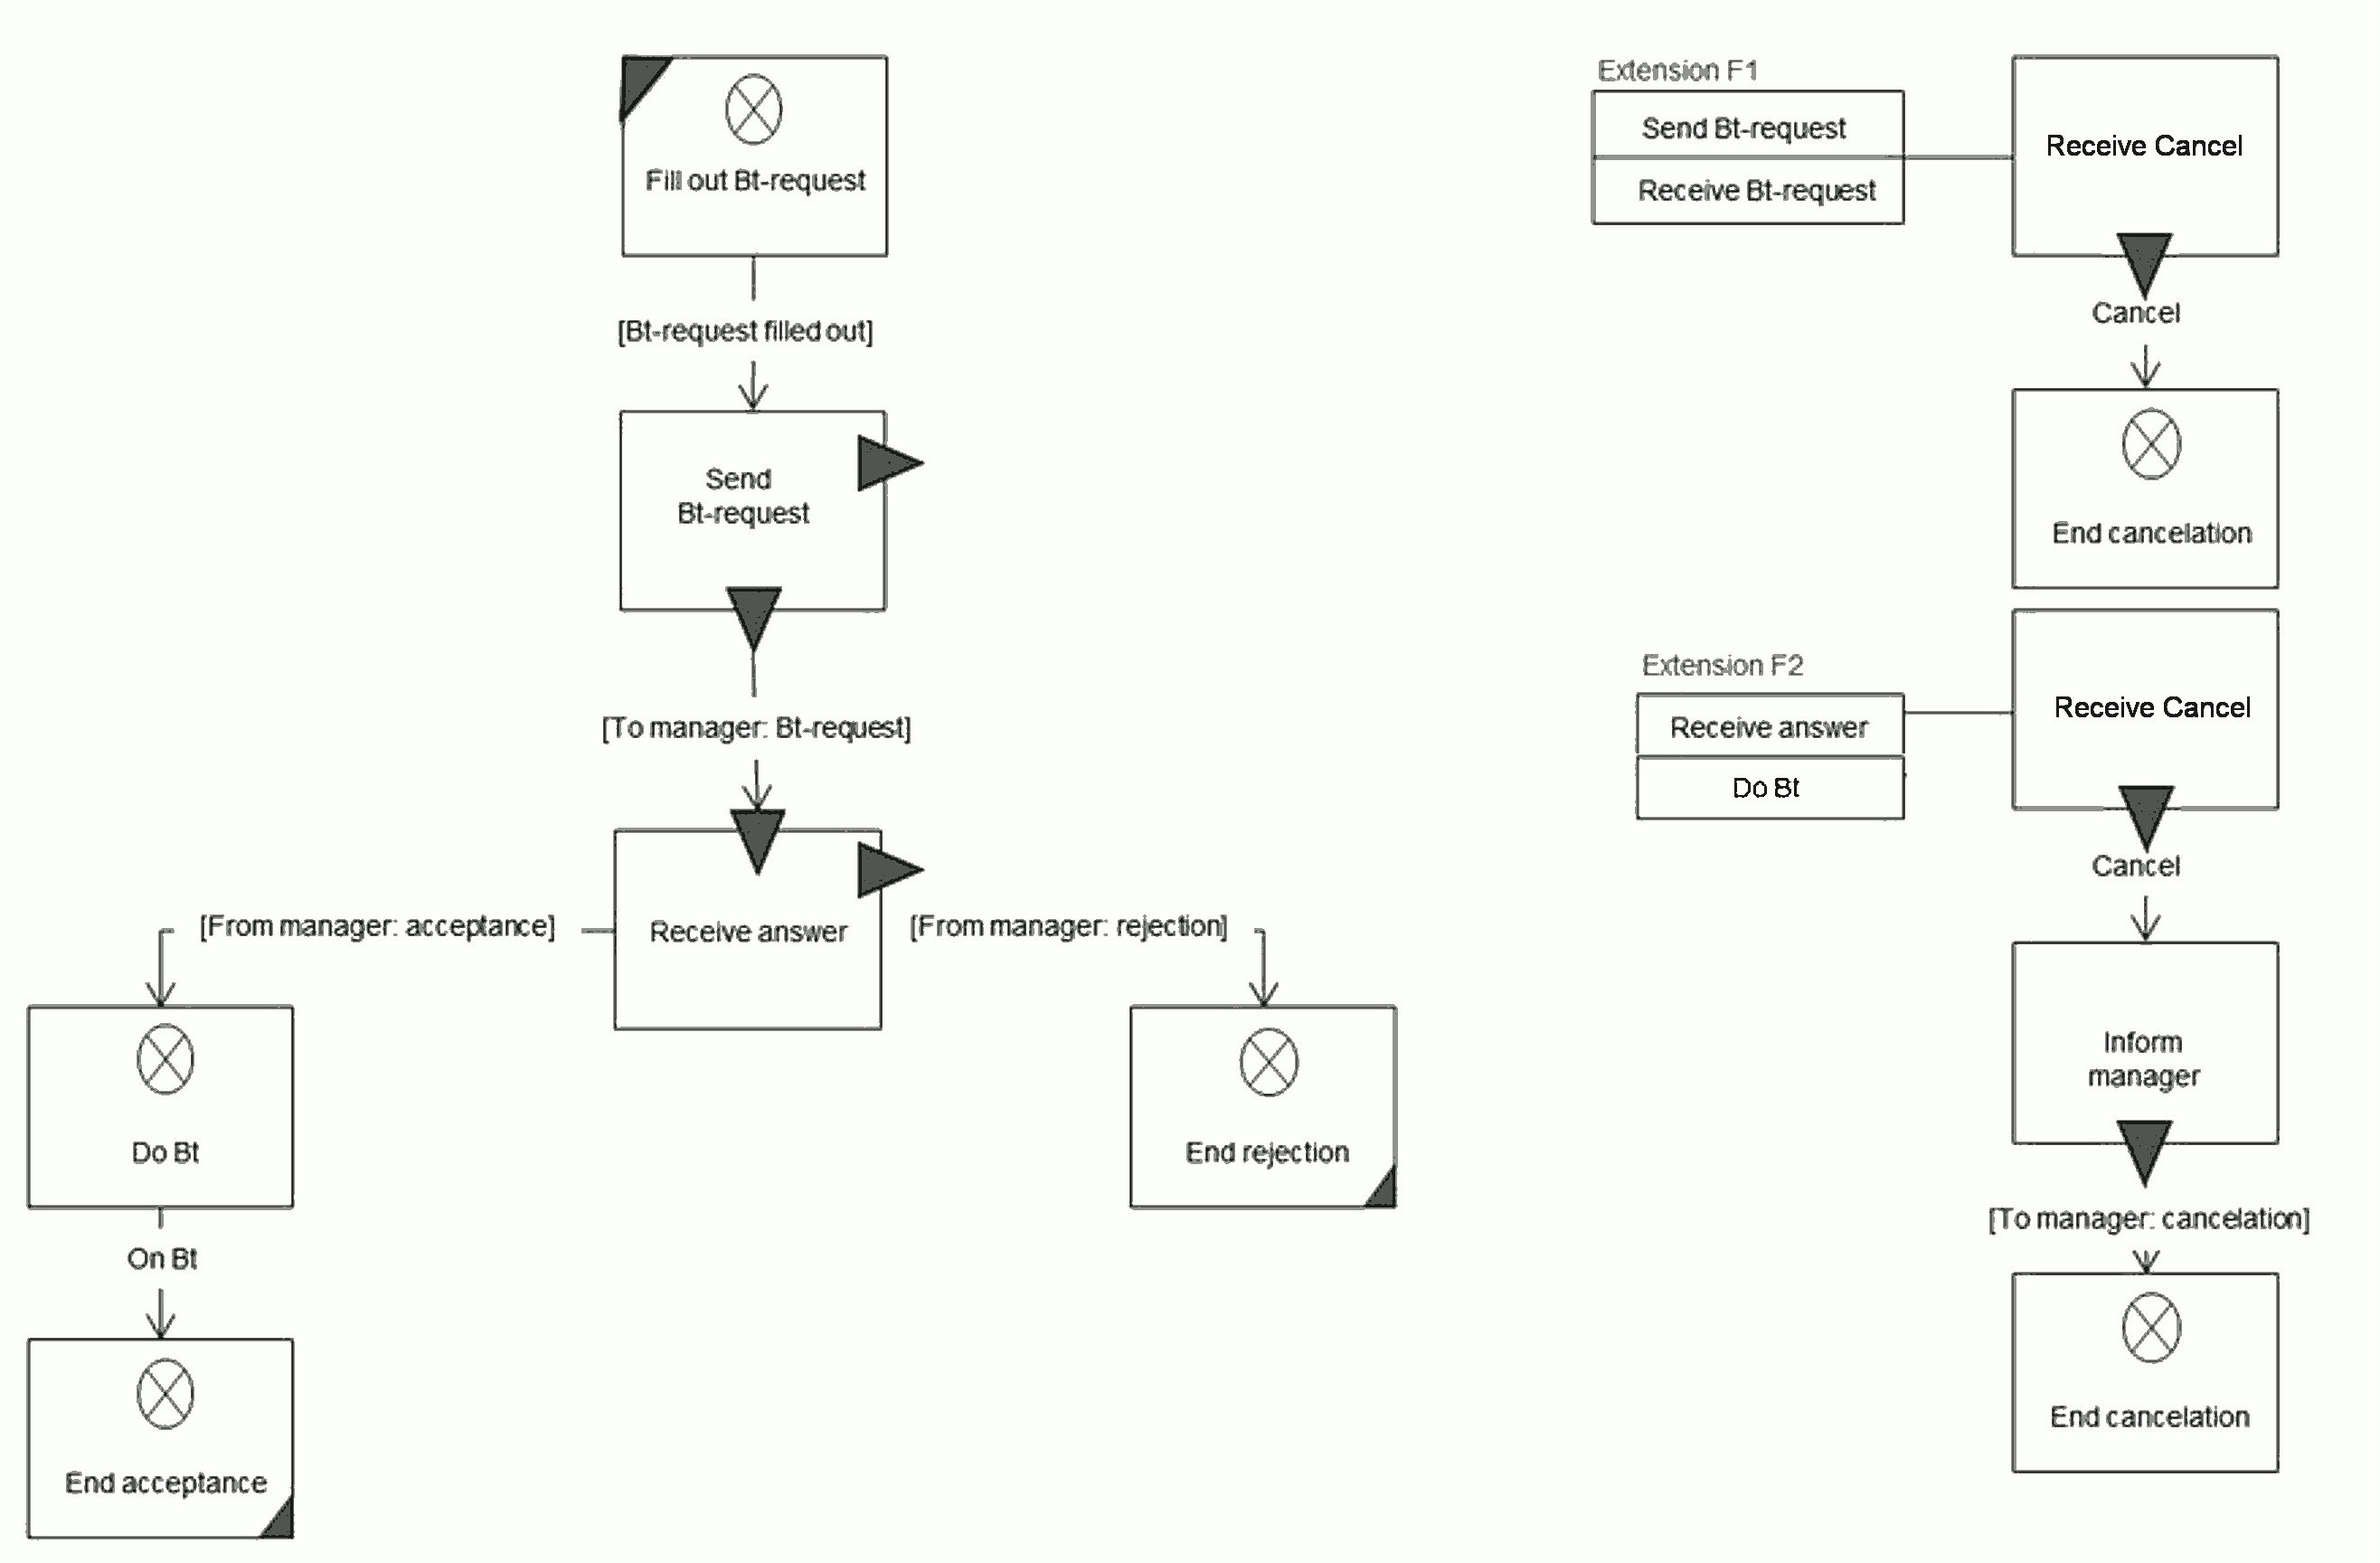
\includegraphics[width=0.7\linewidth]{Figures/Ontology/SubjectBehavior/Extension}
	\caption[Base Behavior and two (separate \textbf{Guard Behaviors} of subject 'employee'.]{Base Behavior and two (separate \textbf{Guard Behaviors} of subject 'employee' setup to guard specific States}
	\label{fig:extension1}
\end{figure}


%Note ME: The following were the original concepts for Guards and Exceptions. They are mostly not valid anymore or have been updated

%\textbf{Exception Handling}---
%Handling of an exception (also termed message guard, message control, message monitoring, message observer) is a behavioral description of a subject that becomes relevant when a specific, exceptional situation occurs while executing a subject behavior specification. It is activated when a corresponding message is received, and the subject is in a state in which it can respond to the exception handling. In such a case, the transition to exception handling has the highest priority and will be enforced.

%Exception handling is characterized by the fact that it can occur in a process in many behavior states of subjects. The receipt of certain messages, e.g., to abort the process, always results in the same processing pattern. This pattern would have to be modeled for each state in which it is relevant. Exception handling causes high modeling effort and leads to complex process models since from each affected state a corresponding transition has to be specified. To prevent this situation, we introduce a concept similar to exception handling in programming languages or interrupt handling in operating systems.

%To illustrate the compact description of exception handling, we use again the service management process with the subject 'service desk' introduced in section 5.6.5. This subject identifies a need for a business trip in the context of processing a customer order—an employee needs to visit the customer to provide a service locally. The subject 'service desk' passes on a service order to an employee. Hence, the employee issues a business trip request. In principle, the service order may be canceled at any stage during processing up to its completion. Consequently, this also applies to the business trip application and its subsequent activities.
    
%Below, it is first shown how the behavior modeling looks without the concept of exception handling. The cancellation message must be passed on to all affected subjects to bring the process to a defined end. Figure \ref{fig:sid-exception} shows the communication structure diagram with the added cancellation messages to the involved subjects.


%A cancellation message can be received by the employee either while filling out the application or while waiting for the approval or rejection message from the manager. Concerning the behavior of the subject 'employee', the state 'response received from manager' must also be enriched with the possible input message containing the cancellation and the associated consequences (see Figure \ref{fig:exceptionhandling}). The verification of whether filing the request is followed by a cancellation is modeled through a receive state with a timeout. In case the timeout is zero, there is no cancellation message in the input pool and the business trip request is sent to the manager. Otherwise, the manager is informed of the cancellation and the process terminates for the subject 'employee'.

%A corresponding adjustment of the behavior must be made for each subject which can receive a cancellation message, including the manager, the travel office, and the interface subject 'travel agent'.

%This relatively simple example already shows that taking such exception messages into account can quickly make behavior descriptions confusing to understand. The concept of exception handling, therefore, should enable supplementing exceptions to the default behavior of subjects in a structured and compact form. 

%Instead of, as shown in Figure \ref{fig:exceptionhandling}, modeling receive states with a timeout zero and corresponding state transitions, the behavioral description is enriched with the exception handling 'service cancellation'. Its initial state is labeled with the states from which it is branched to, once the message 'service cancellation' is received. In the example, these are the states 'fill out Bt-request' and 'receive answer from manager'. Each of them is marked by a triangle on the right edge of the state symbol. The exception behavior leads to an exit of the subject after the message 'service cancellation' has been sent to the subject 'manager'.

%A subject behavior does not necessarily have to be brought to an end by an exception handling; it can also return from there to the specified default behavior. Exception handling behavior in a subject may vary, depending on from which state or what type of message (cancellation, temporary stopping of the process, etc.) it is called. The initial state of exception handling can be a receive state or a function state.

%Messages, like 'service cancellation', that lead to exception handling always have higher priority than other messages. This is how modelers express that specific messages are read in a preferred way. For instance, when the approval message from the manager is received in the input pool of the employee, and shortly thereafter the cancellation message, the latter is read first. This leads to the corresponding abort consequences.

%Since now additional messages can be exchanged between subjects, it may be necessary to adjust the corresponding conditions for the input-pool structure. In particular, the input-pool conditions should allow storing an interrupt message in the input pool. To meet organizational dynamics, exception handling and extensions are required. They allow taking not only discrepancies but also new patterns of behavior, into account.

\subsection{Subject Specific Macros}

Quite often, a certain behavior pattern occurs repeatedly within a subject. This happens in particular when in various parts of the process identical actions need to be performed. If only the basic constructs are available to this respect, the same sub- behavior needs to be described many times.

Instead, a repeated behavior fragment can be defined as a so-called \PASSModelElement{Macro Behavior}. Such a Macro Behavior then can be called from different states in an SBD as often as required. Thus, variations in behavior can be consolidated, and the overall behavior can be significantly simplified.

To illustrate with an example an simple order processing is being used. Figure \ref{fig:macrobehavior} shows the SBD of a macro behavior that describes the activities to handle customer orders. After placing the 'order', the customer receives an order confirmation; once the 'delivery' occurs, the delivery status is updated. Instead of ending in a normal end state, the Macro Behavior ends in a Generic-Return-To-Origin-Reference, that refers the execution back to the state from which this Macro Behavior was called. This generic approach is necessary, since such a call can happen from multiple times from multiple different states during the execution of the overall process model. 

\begin{figure*}[htbp]
	\centering
	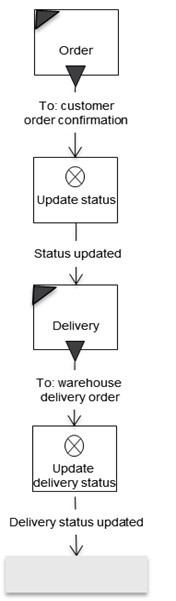
\includegraphics[width=0.2\linewidth]{Figures/Ontology/SubjectBehavior/MacroBehavior}
	\caption[Behavior macro class 'request for approval']{Behavior macro class 'request for approval'}
	\label{fig:macrobehavior}
\end{figure*}

A call to a Macro Behavior is conceptualized similar to an advanced function call or refinement - an addition to one of the states of another SBD. No restrictions have been made regarding the type of the state. A Macro calling state is therefor also called a \PASSModelElement{Macro State}.

Usually the Macro calling is a replacement for the internal function of a Do-State, or the additional function of Receive and Send states. Calling to the Macro happens before executing the rest. If execution of the Macro Behavior produces results that influence e.g. the choice of a certain branch to continue, this must be reflected in a change in the internal data store of a subject and subsequently be evaluated in the outgoing transitions of the Macro State. 

%Figure \ref{fig:macrousage} shows a subject behavior in which the modeler uses the macro 'order processing' to model both a regular order (with purchase order), as well as a call order.

%The icon for a macro is a small table, which can contain multiple columns in the first line for different start states of the macro. The valid start state for a specific case is indicated by the incoming edge of the state transition from the calling behavior. The middle row contains the macro name, while the third row again may contain several columns with possible output transitions, which end in states of the surrounding behavior.

%The left branch of the behavioral description refers to regular customer orders. The embedded macro is labeled correspondingly and started with the status 'order', namely through linking the edge of the transition 'order accepted' with this start state. Accordingly, the macro is closed via the transition 'delivery status updated'.

%The right embedding deals with call orders according to organizational frameworks and frame contracts. The macro starts therefore in the state 'delivery'. In this case, it also ends with the transition 'delivery status updated'.

%\begin{figure}[htbp]
%	\centering
%	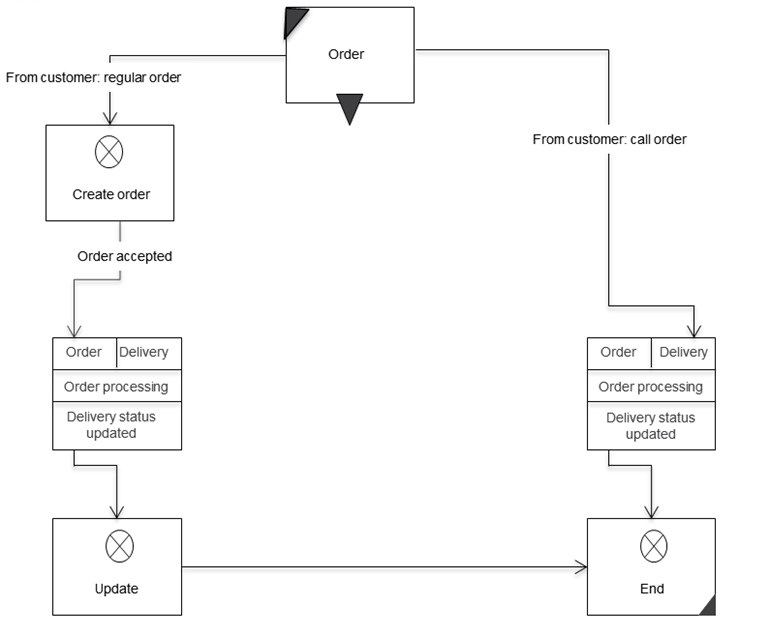
\includegraphics[width=0.6\linewidth]{Figures/Ontology/SubjectBehavior/MacroUsage}
%	\caption[Subject behavior for order processing with macro integration]{Subject behavior for order processing with macro integration}
%	\label{fig:macrousage}
%\end{figure}

%Similar subject behavior can be combined into macros. When being specified, the environment is initially hidden, since it is not known at the time of modeling.



%\textbf{Behavior Extensions}---
%When exceptions occur, currently running operations are interrupted. This can lead to inconsistencies in the processing of business objects. For example, the completion of the business trip form is interrupted once a cancellation message is received, and the business trip application is only partially completed. Such consequences are considered acceptable, due to the urgency of cancellation messages. In less urgent cases, the modeler would like to extend the behavior of subjects in a similar way, however, without causing inconsistencies. This can be achieved by using a notation analogous to exception handling. Instead of denoting the corresponding diagram with 'exception', it is labeled with 'extension'.

%Behavior extensions enrich a subject's behavior with behavior sequences that can be reached from several states equivocally.

%For example, the employee may be able to decide on his own that the business trip is no longer required and withdraw his trip request. Figure \ref{fig:extension2} shows that the employee can cancel a business trip request in the states 'send business trip request to manager' and 'receive answer from manager'. If the transition 'withdraw business trip request' is executed in the state 'send business trip request to manager', then the extension 'F1' is activated. It leads merely to canceling of the application. Since the manager has not yet received a request, he does not need to be informed.

%In case the employee decides to withdraw the business trip request in the state 'receive answer from manager', then extension 'F2' is activated. Here, first the supervisor is informed, and then the business trip is canceled.

%\begin{figure}[htbp]
%	\centering
%	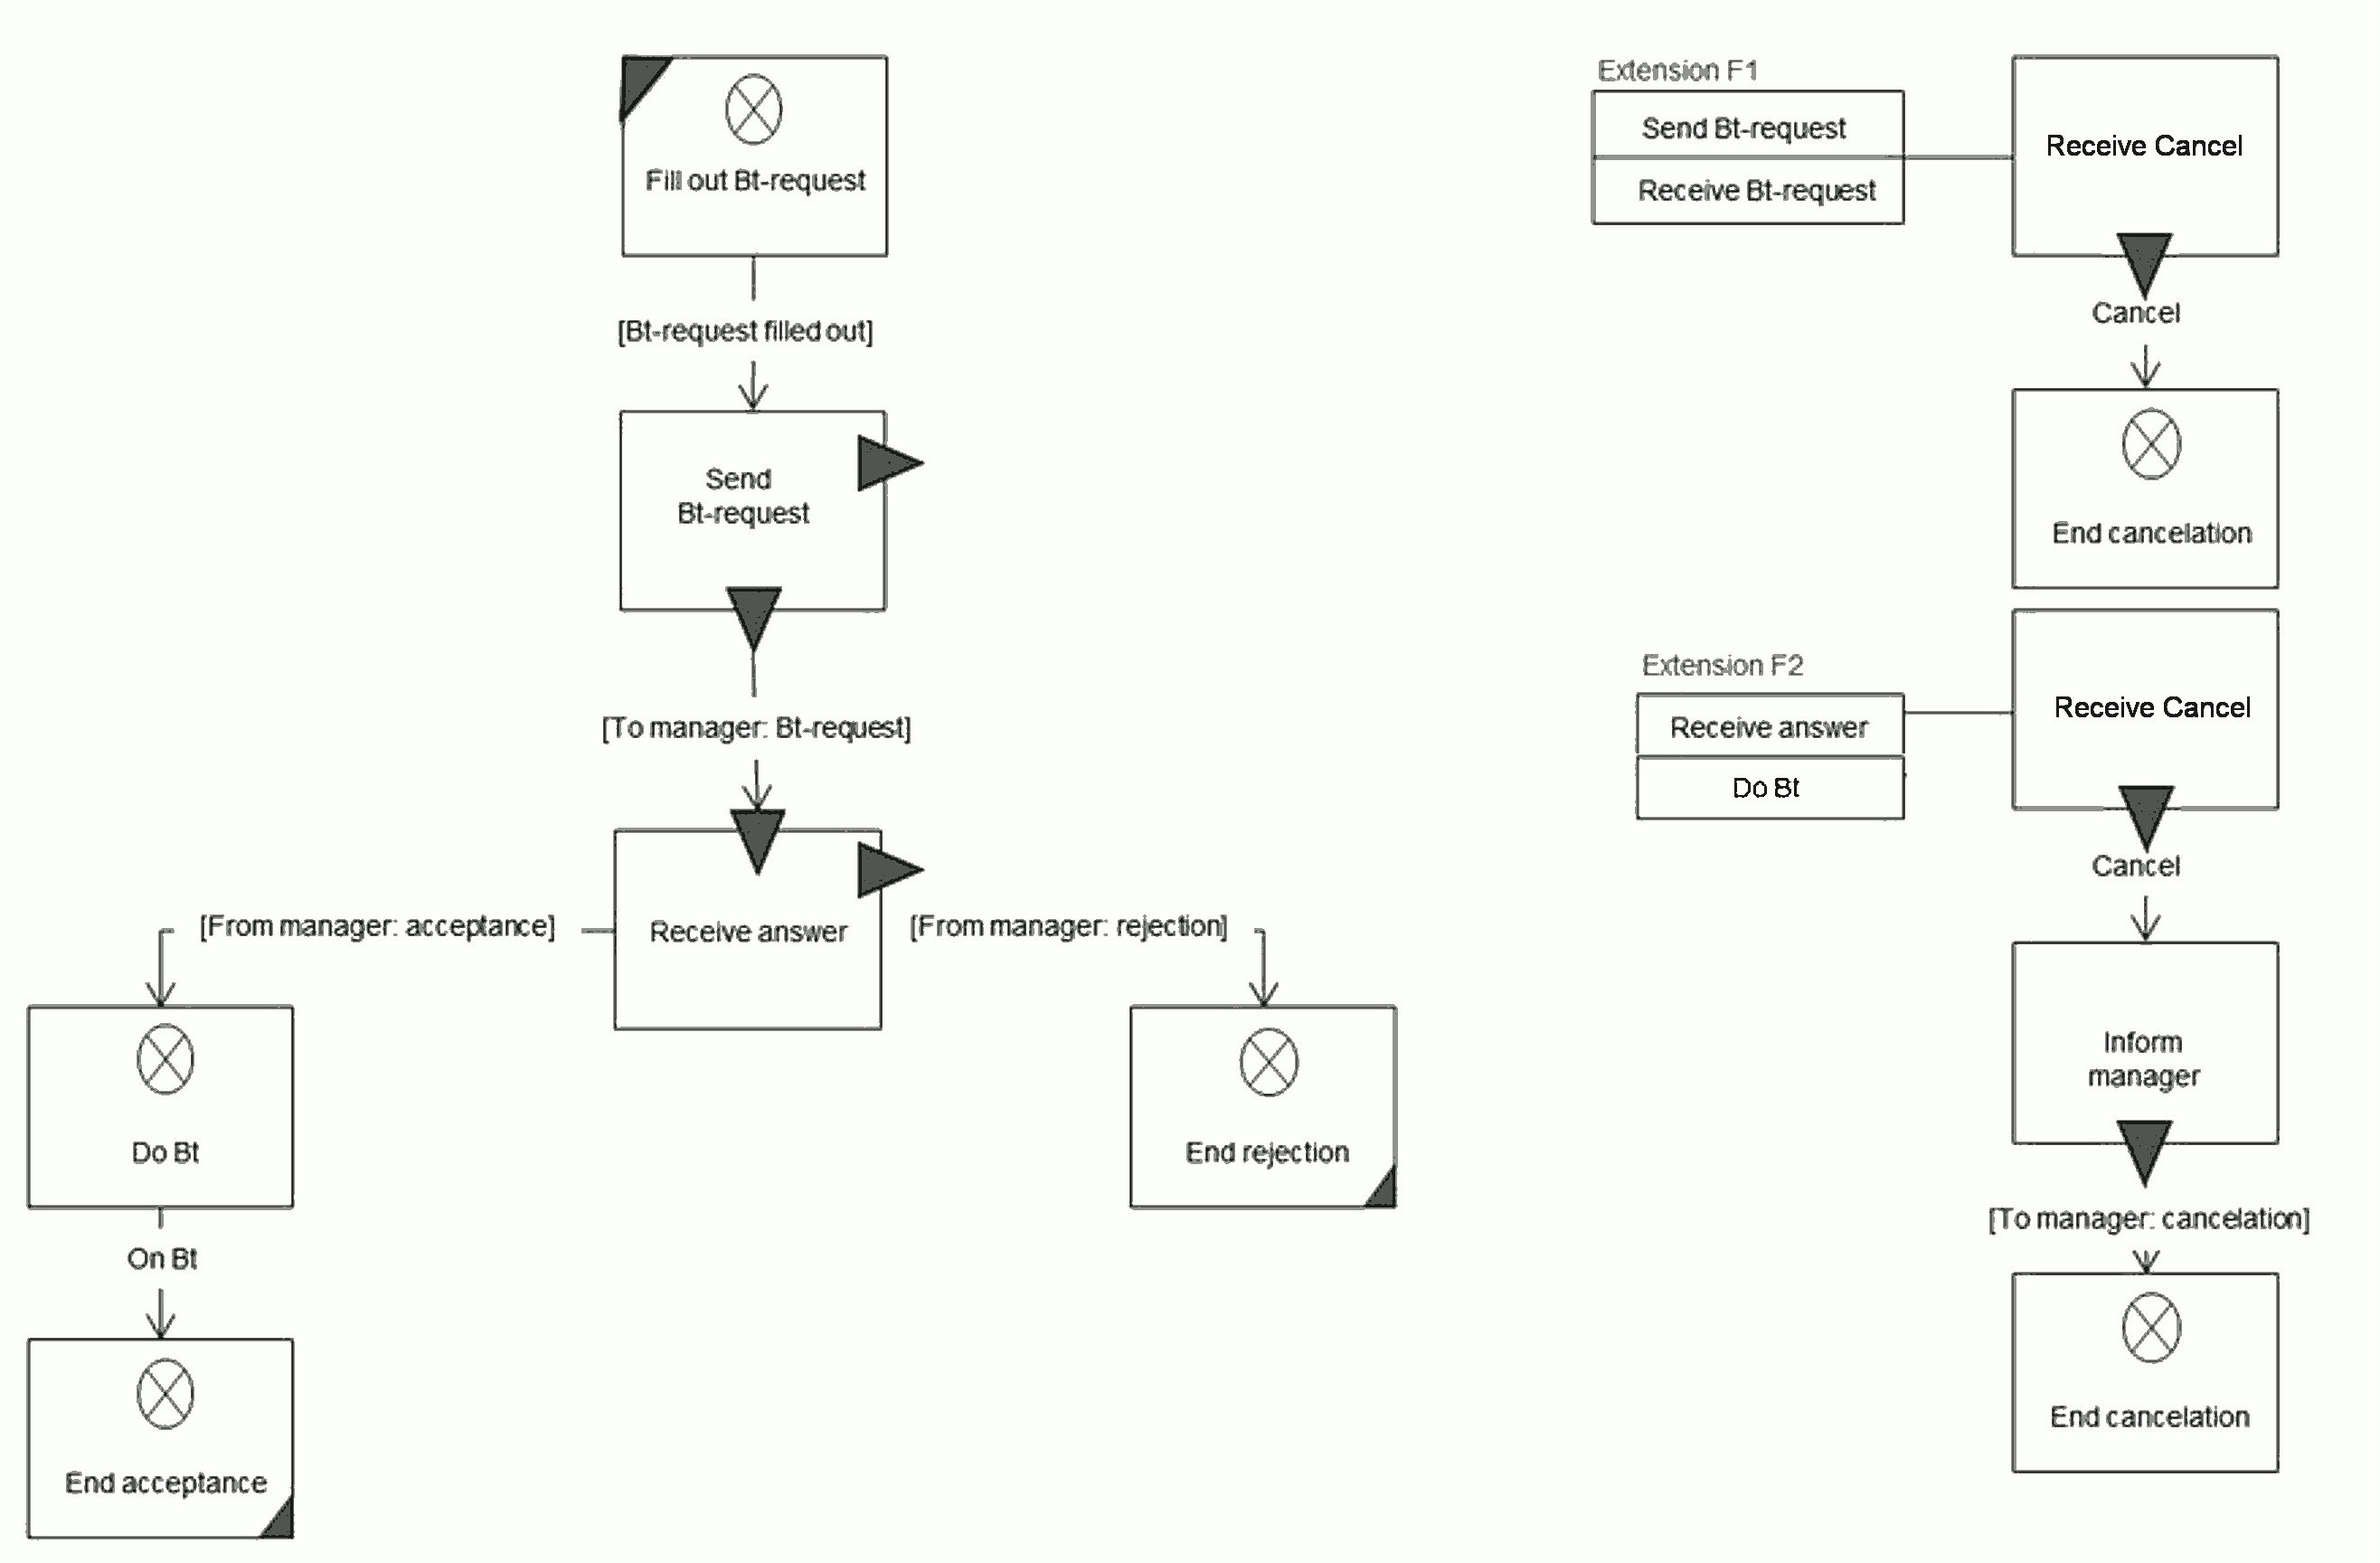
\includegraphics[width=0.7\linewidth]{Figures/Ontology/SubjectBehavior/Extension}
%	\caption[Subject behavior of employee with behavior extensions]{Subject behavior of employee with behavior extensions}
%	\label{fig:extension2}
%\end{figure}




